\section{The Hall A High Resolution Spectrometer}

Hall A has two 4 GeV/c High Resolution Spectrometers (HRSs). In order to achieve Hall A's stated goal of $1\%$ absolute cross section accuracy, the HRSs were designed to have $10^{-4}$ particle momentum resolution and $0.1$ mrad in scattering angle resolution. 

Each HRS has four superconducting magnets: three cos$\left(2\theta\right)$ and a racetrack coil dipole. Utilizing a QQDQ magnet setup, each HRS has a $45\degree$ bending angle in a vertical bending plane. Each HRS has a similar, but unique, detector package that accommodates precise tracking and particle identification (PID).

\subsection{Detectors}

Each arm consists of a pair of Vertical Drift Chambers (VDCs), two scintillator planes, a gas cherenkov, and two leaded glass calorimeters.

\subsubsection{Vertical Drift Chambers}

Each arm has two VDCs at the entrance to the detector stack. These chambers are oriented parallel to the horizontal plane of the hall, $45\degree$ to the detector stack, and $90\degree$ to each other. Each chamber has two wire planes in a UV formation that are separated by 335 mm. In each plane there are 368 wires with a wire spacing of 4.24 mm. This setup gives a position resolution of 100 $\mu$m and an angular resolution of 0.5 mrad.

\subsubsection{Scintillator Planes}

Each HRS has two scintillator planes that were used for MARATHON: S0 and S2. These two planes sandwich the Gas Cherenkov. The scintillators are plastic paddles with a Photomultiplier Tube (PMT) on each end. S0 consists of a single paddle with the PMTs on located on the top and bottom. S2 consists of 16 paddles with the PMTs on the left and right.

The scintillators are used for timing the VDC signal and for producing triggers.

\subsubsection{Gas Cherenkov}

The CO2 Gas Cherenkov is the first PID detector in the HRS. The Cherenkov chamber is filled with C02 at atmospheric pressure. This gives 4.8 GeV/\textit{c} threshold for pion detection. There are ten spherical mirrors each with a PMT. The radiator length is 80 cm for the LHRS and 130 cm for the RHRS.

Analyzing the ADC sum or the ten PMTs provides clear identification of electrons.

\subsubsection{Leaded Glass Calorimeters}

Both arms have two leaded glass calorimeters, known as the preshower and shower detectors.

In the LHRS, the preshower and shower blocks are all perpendicular to the path of the particle. Both layers have are comprised of 34 blocks at alternate in size between 15 cm x 15 cm x 30 cm and 15 cm x 15 cm x 35 cm.

In the RHRS, the preshower blocks are perpendicular to the path of the particle while the shower blocks are parallel to the path of the particle. The preshower layer is composed of 48 blocks that measure 10 cm x 10 cm x 35 cm. The shower layer is composed of 80 blocks that measure 15 cm x 15 cm x 35 cm.

\begin{figure}
	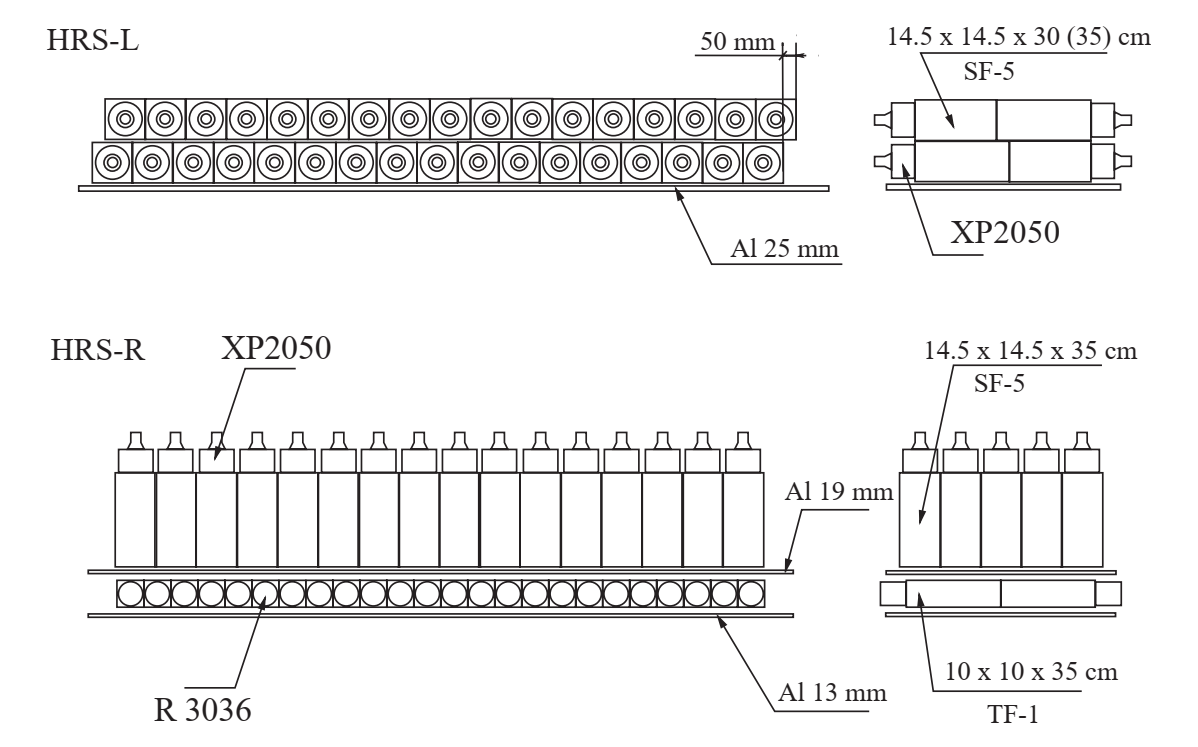
\includegraphics[width=\linewidth]{./chap2-exp/fig/shower_layout.png}
	\caption{Layout of the shower block. Particles enter from the bottom of the page. Left is top-view. Right is side-view. \cite{HANIM}}
	\label{shower_layout}
\end{figure}